\documentclass[main.tex]{subfiles}
\begin{document}

\section{User Guide}
\label{sec:userguide}
YANF is a cookie and request blocker for android phones. The benefit of YANF is that t works globally for all apps sending request via HTTP and HTTPS. This guide will go through the basics of using YANF. The guide contains the following sections

\begin{itemize}
    \item \nameref{UG-YANF-UI}
    \item \nameref{sec:YANF_First}
    \item \nameref{UG-BlockingCookies}
    \item \nameref{UG-BlockingAds}
    \item \nameref{UG-Statistics}
    \item \nameref{sec:UG-turnOff}
\end{itemize}

\subsection{YANF UI}
\label{UG-YANF-UI}
The YANF user interface(UI) is build from simple components giving the user easy access to the different features. The UI can be seen in \autoref{fig:ui}.

\begin{figure}[H]
    \centering
    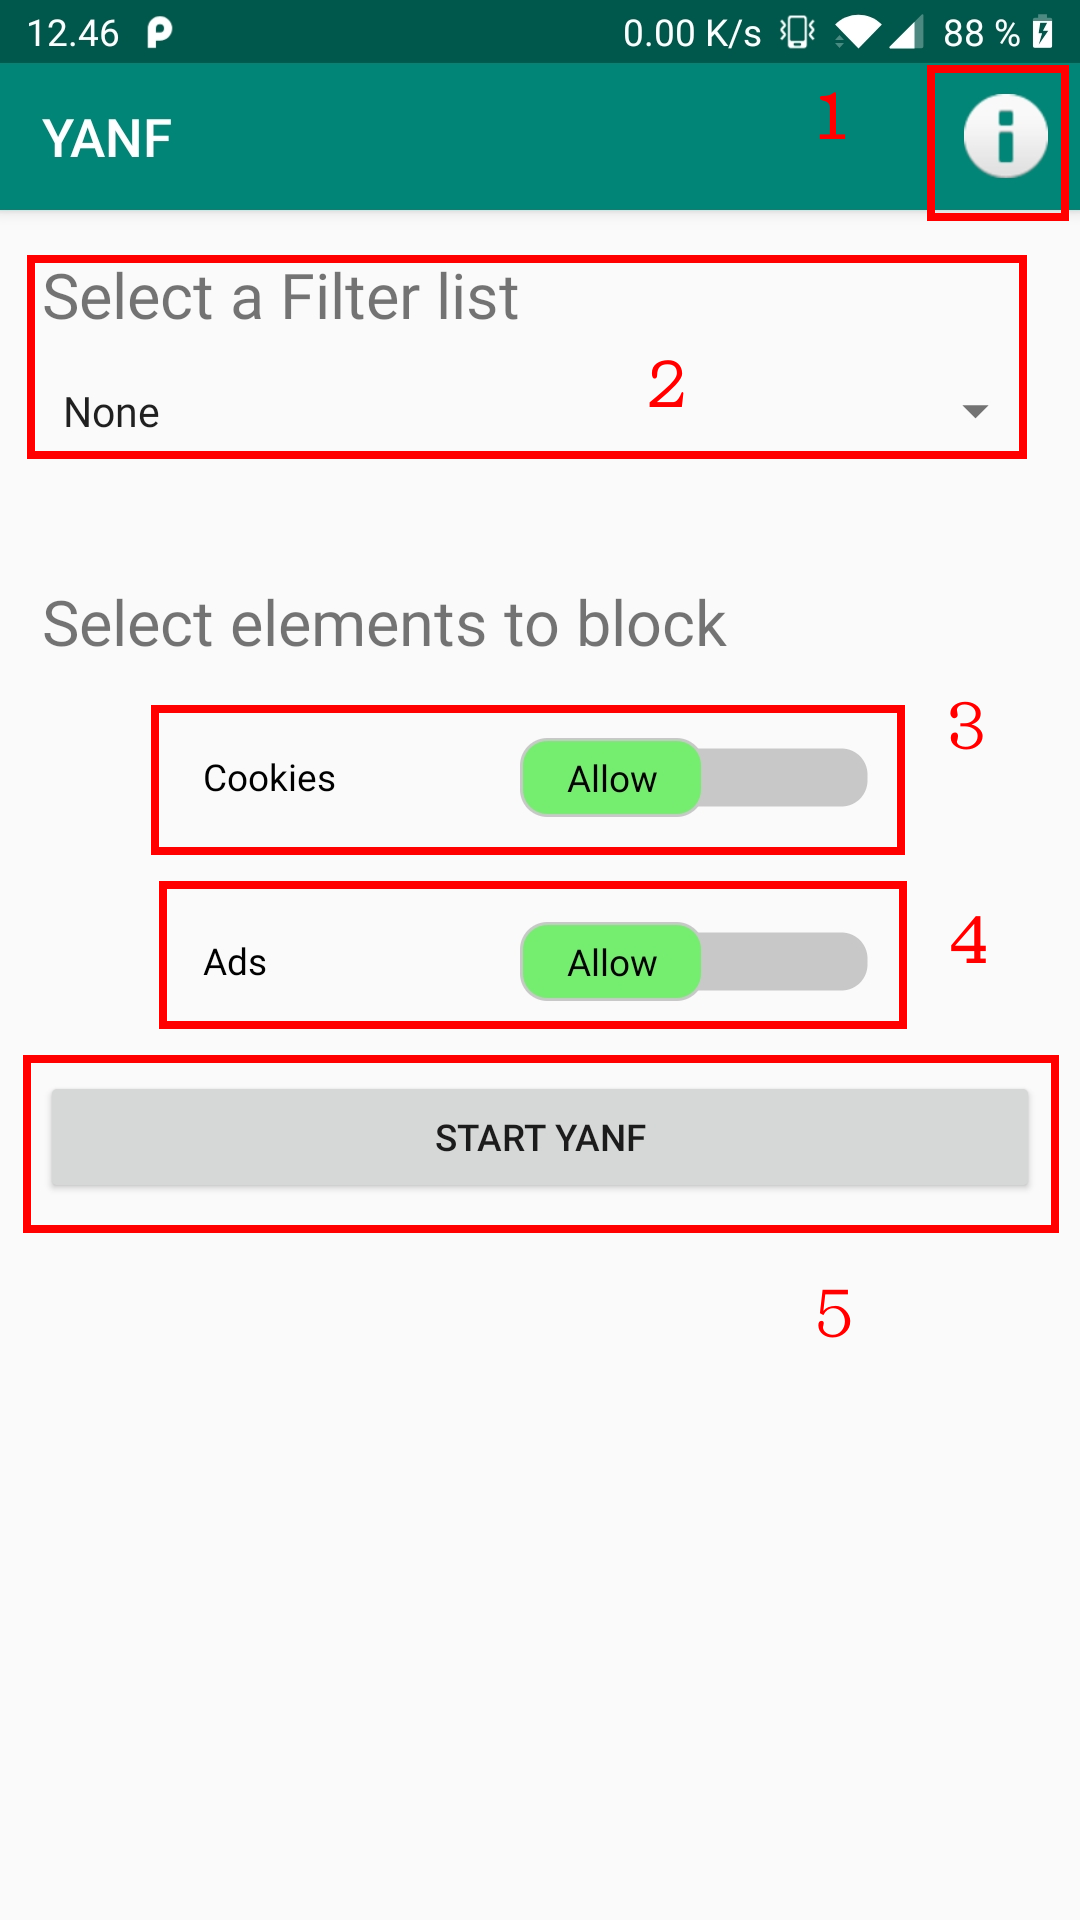
\includegraphics[width=0.3\textwidth]{1_Appendix/UI/yanf_numbered.png}
    \caption{YANF User Interface}
    \label{fig:ui}
\end{figure}

Descriptions for the different elements marked in \autoref{fig:ui} can be found in the list below:

\begin{enumerate}
    \item Switches view to filter statistics
    \item Drop down to select what to filter
    \item Toggle to enable the blocking of cookies for the selected filter
    \item Toggle to enable the blocking of requests for the selected filter
    \item Button to start YANF
\end{enumerate}

\subsection{Starting YANF the first time}
\label{sec:YANF_First}
When the start button is pressed the first time, the user will be prompted to install a certificate. This is done by pressing \textit{ok} as shown in \autoref{fig:ui_ssl}. After the certificate is installed, YANF can be started.

\begin{figure}[H]
    \centering
    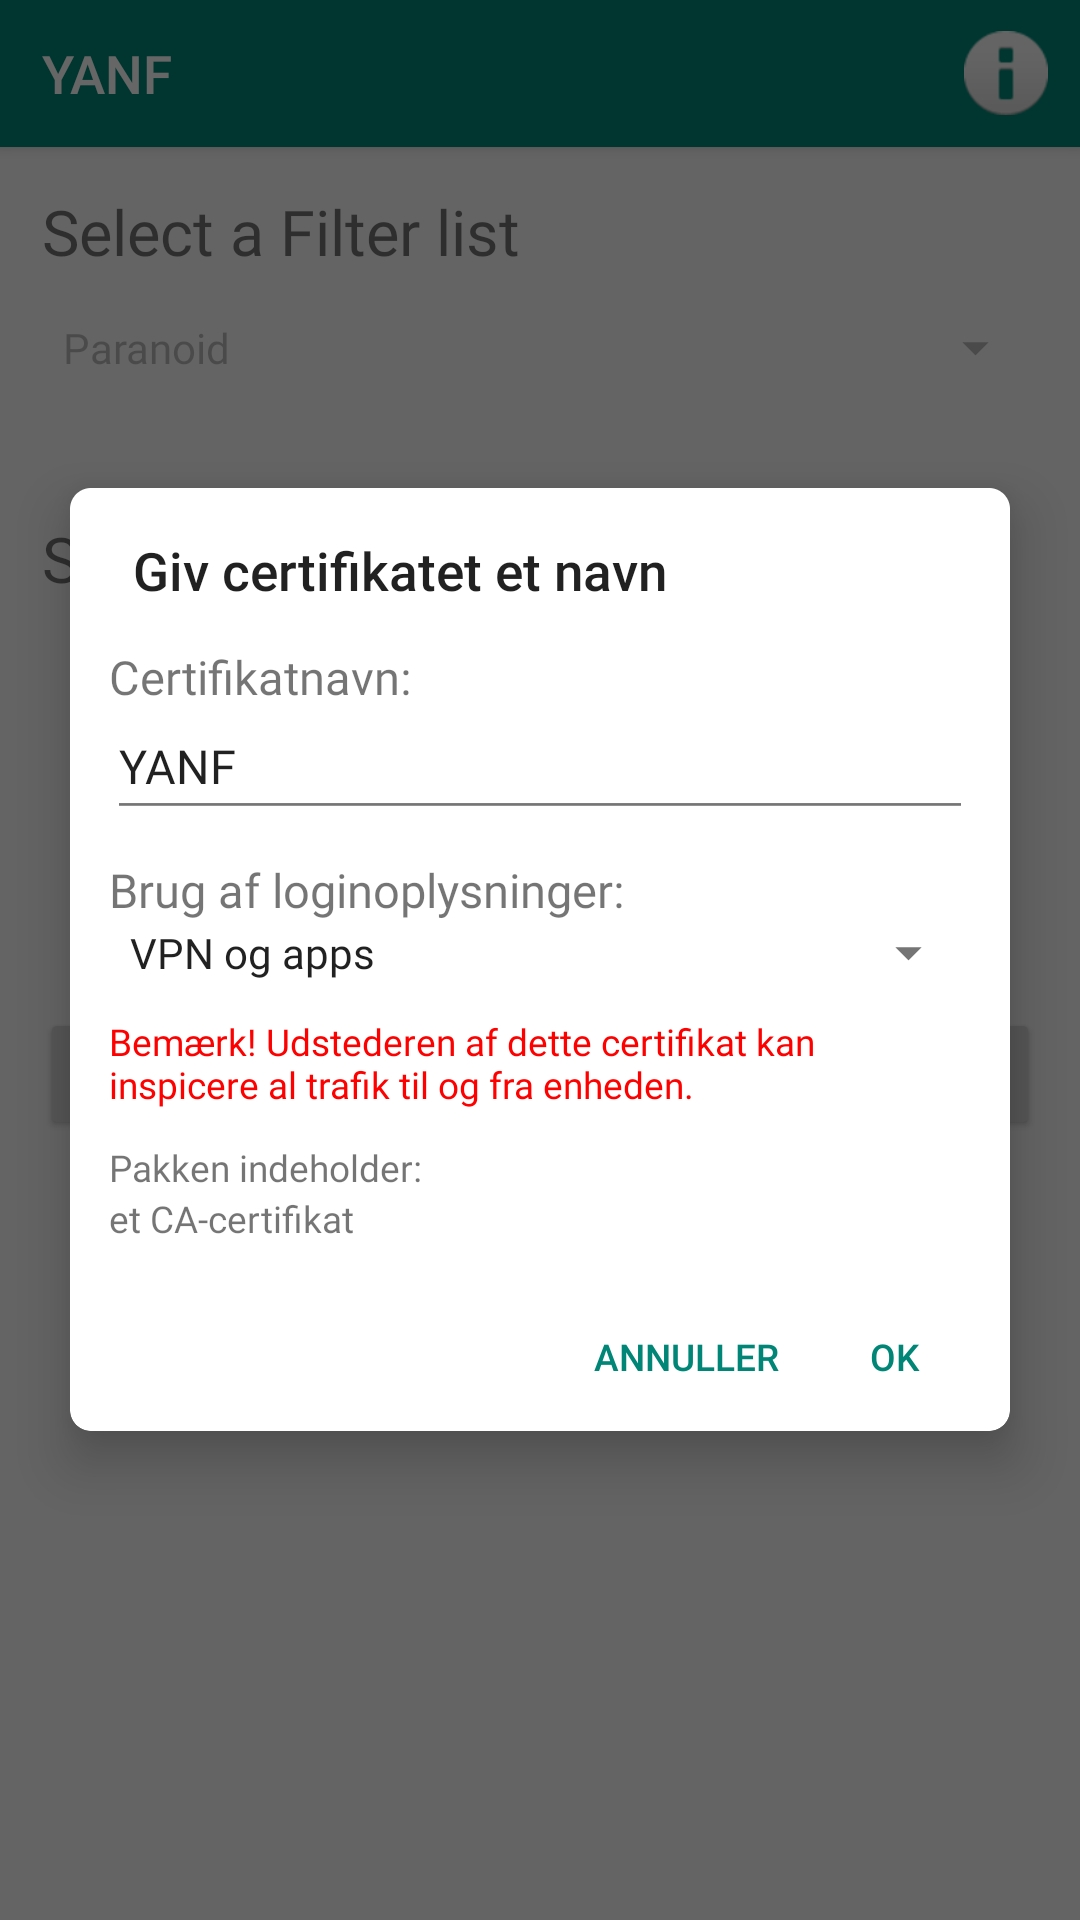
\includegraphics[width=0.3\textwidth]{1_Appendix/UI/install_certificate.jpg}
    \caption{Certificate installation}
    \label{fig:ui_ssl}
\end{figure}

\subsection{Blocking Cookies}
\label{UG-BlockingCookies}
In order to block cookies, the user selects a filter. Then enables the cookie blocking by switching the cookie toggle button. The UI will look as \autoref{fig:ui_cookie} if the \textit{paranoid} filter is selected. Start YANF by pressing the start button.

\begin{figure}[H]
    \centering
    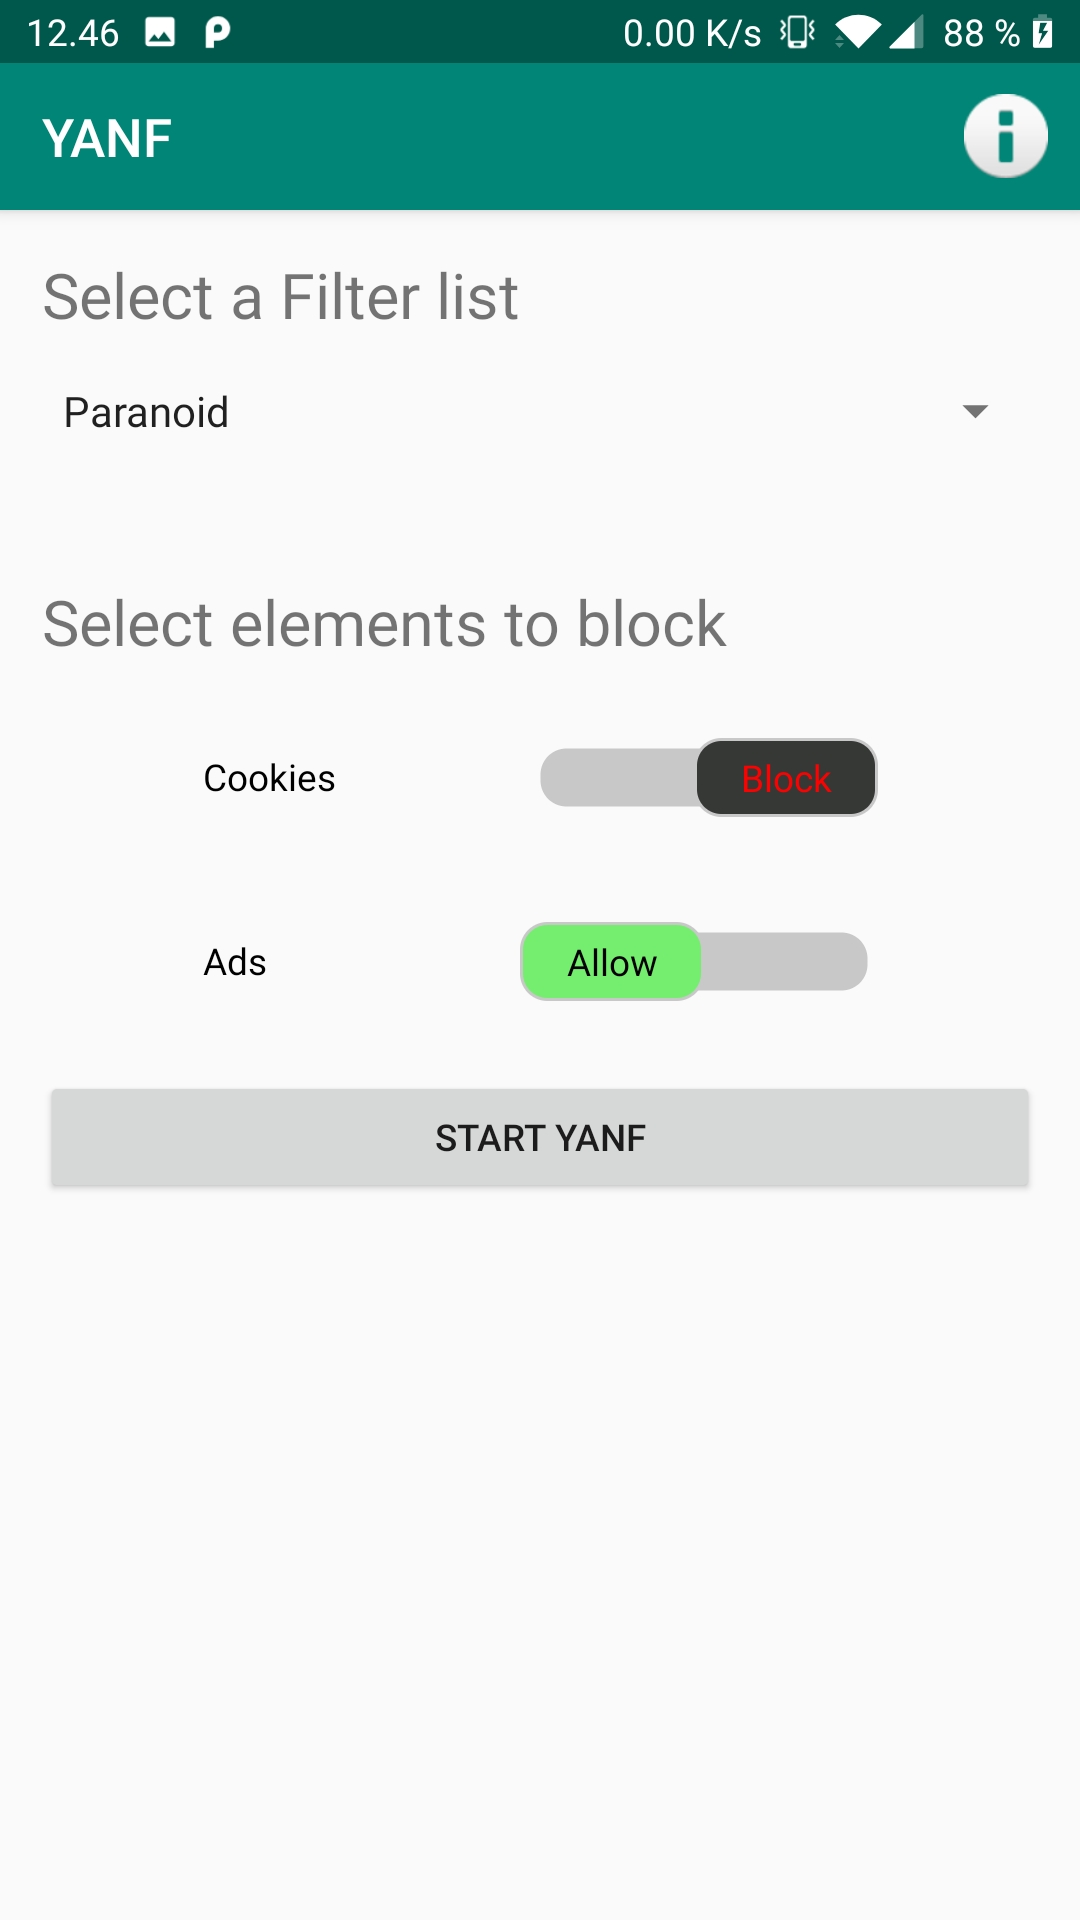
\includegraphics[width=0.3\textwidth]{1_Appendix/UI/cookie_on.jpg}
    \caption{Start cookie blocking}
    \label{fig:ui_cookie}
\end{figure}


\subsection{Blocking Ads}
\label{UG-BlockingAds}
In order to block ads completely, the user selects a filter. Then enables the ad blocking by switching the ads toggle button. The UI will look as \autoref{fig:ui_ads} if the \textit{paranoid} filter is selected. Start YANF by pressing the start button.

\begin{figure}[H]
    \centering
    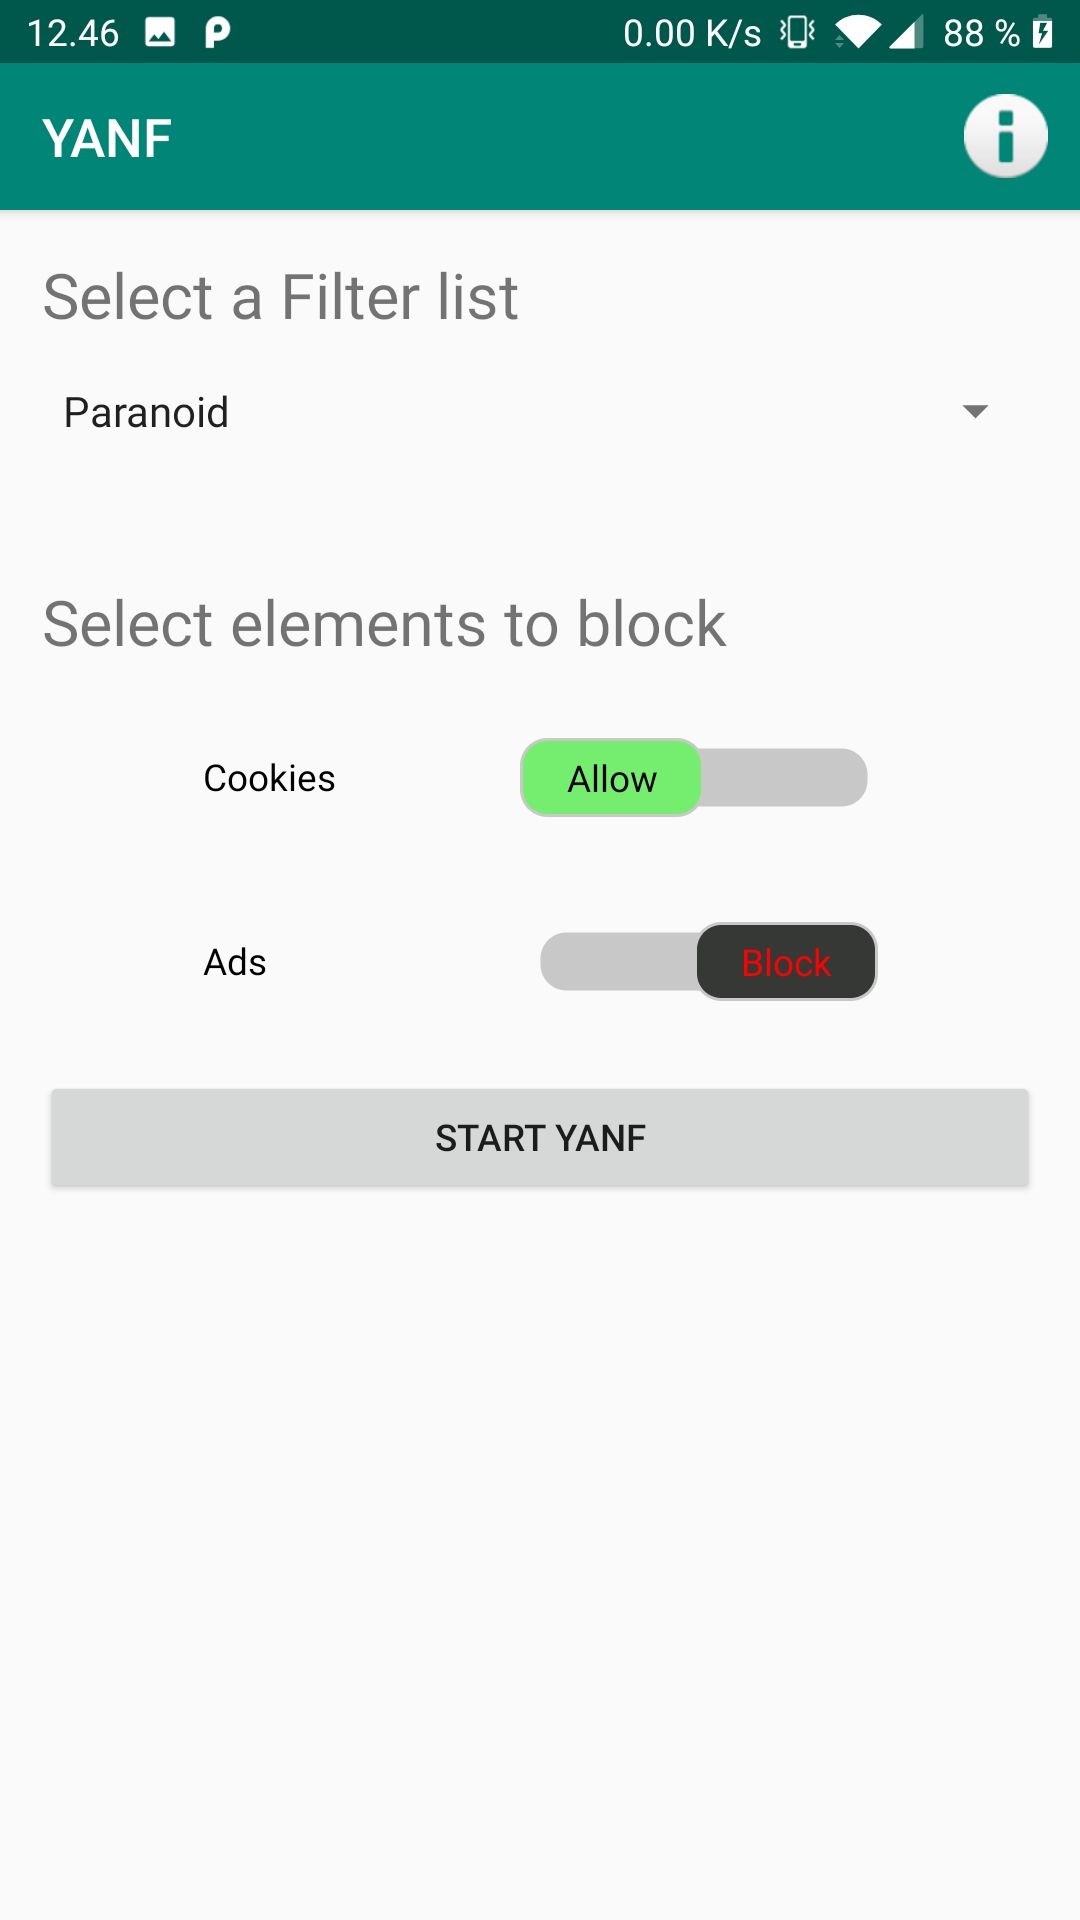
\includegraphics[width=0.3\textwidth]{1_Appendix/UI/ads_on.jpg}
    \caption{Start ad blocking}
    \label{fig:ui_ads}
\end{figure}

\subsection{Using Statistics}
\label{UG-Statistics}
The user has the option of showing the statistics gathered from the use of YANF. The statistics is accessed by pressing button 1 shown in \Smartref{UG-YANF-UI} followed by pressing the \textit{"Statistics"} button. The statistics is a list of domains filtered off by YANF. The list also includes the number of times a domain has been blocked. To update the list, press the \textit{Statistics} button again. The list is reset each time YANF is turned off. An example of how the statistics look can be seen in \autoref{fig:ui_statistic}.

\begin{figure}[H]
    \centering
    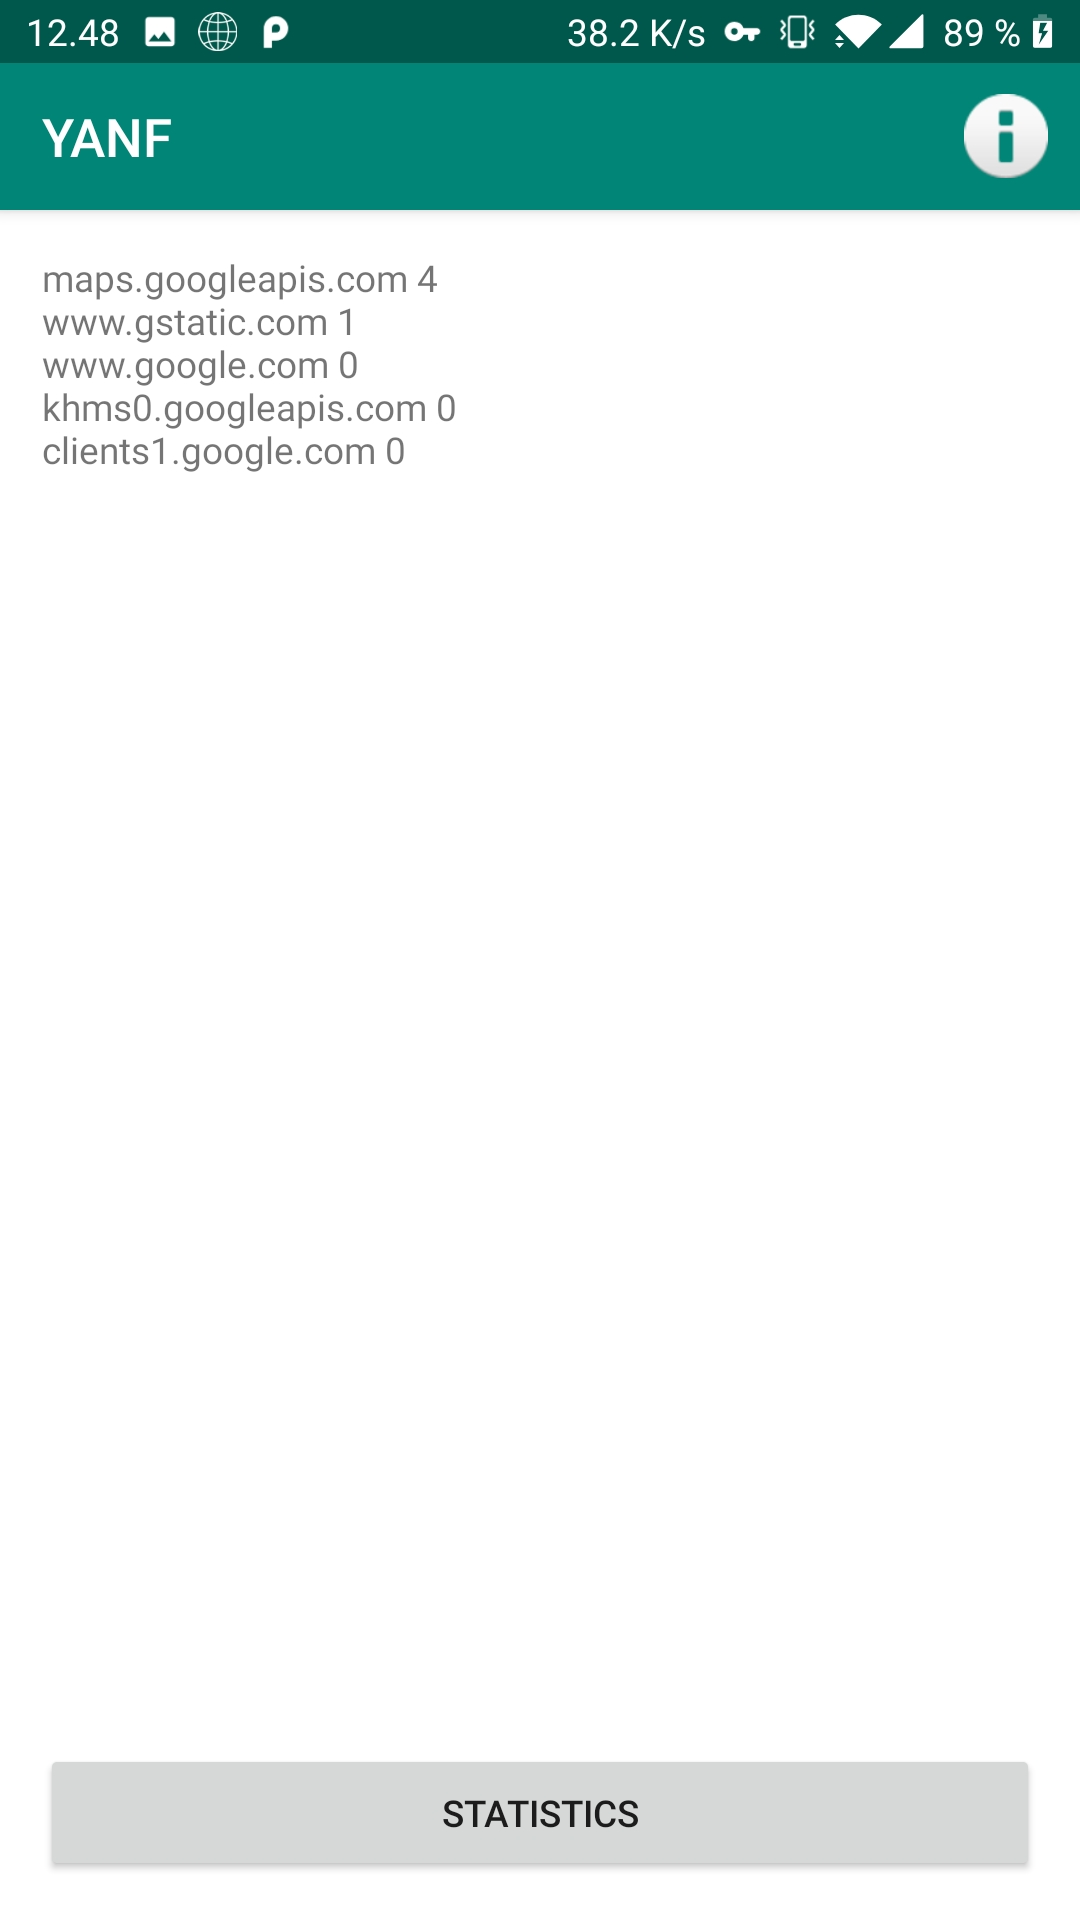
\includegraphics[width=0.3\textwidth]{1_Appendix/UI/stats.jpg}
    \caption{YANF filtering statistics}
    \label{fig:ui_statistic}
\end{figure}

\subsection{Turning off YANF}
\label{sec:UG-turnOff}
YANF can be turned off by pressing the button with the text \textit{"Stop YANF"}, as seen in \autoref{fig:ui_stop}.

\begin{figure}[H]
    \centering
    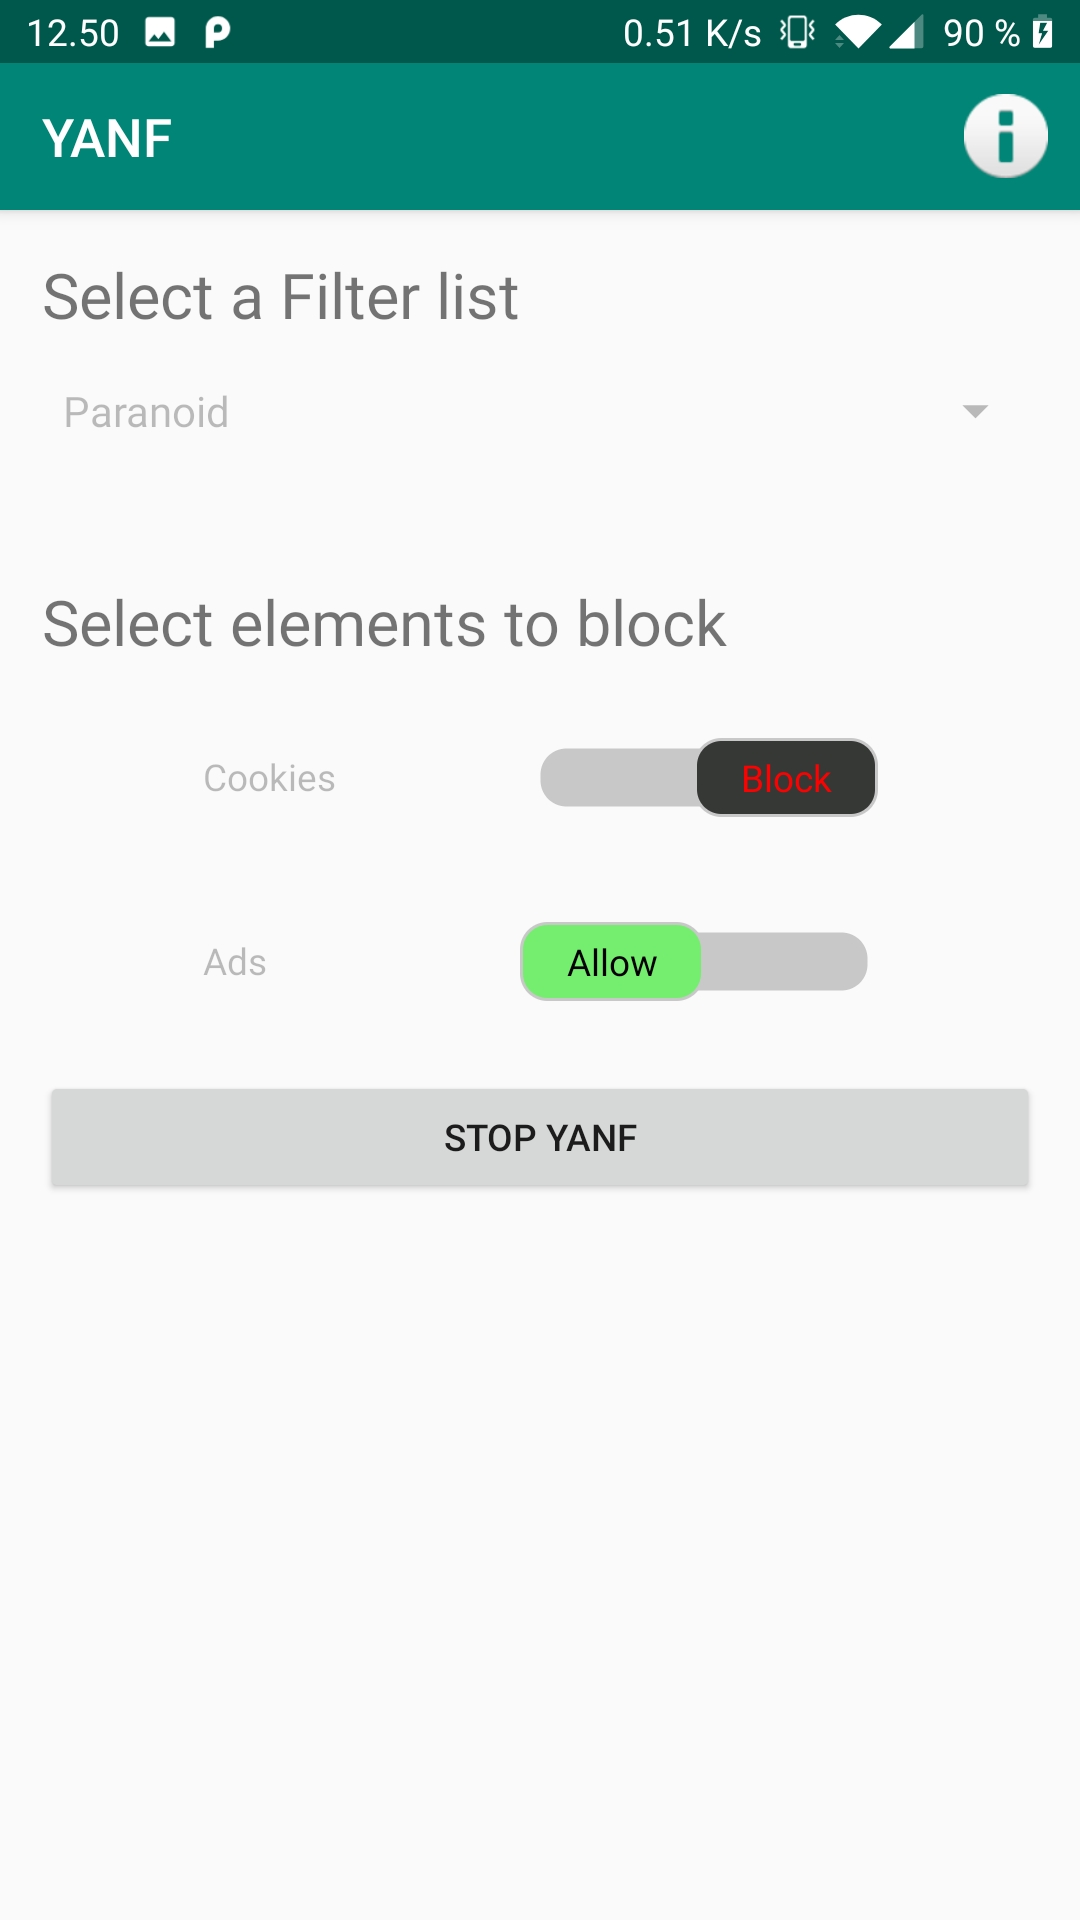
\includegraphics[width=0.3\textwidth]{1_Appendix/UI/yanf_run.png}
    \caption{YANF running}
    \label{fig:ui_stop}
\end{figure}

\end{document}